\subsection{Boundary integrals, formerly `DeLeffe'}
\label{sss:aquagpusph:boundaries:DeLeffe}
%
Boundary integrals is the newest method to compute boundary conditions, and the implementation method is similar
to `ElasticBounce boundary' described at section \ref{sss:aquagpusph:boundaries:elasticbounce}.\\
%
In figure \ref{fig:aquagpusph:DeLeffeScheme} a boundary integrals scheme is shown. In original DeLeffe's boundaries
integral development, oriented to 2D applications, an analytic solution of the integral, with a discretized
version of fields, is purposed for full integration line (green highlighted on the image). In \NAME each vertex
is associated to a wall area, then not only the field is discretized but also the integral as well, with a little
bit worst result, but allowing to use this method in 3D simulations too.\\
%
In order to can converge the discretized boundary integral to the analytical one, you can set more vertexes with
smaller areas, but be mindful that the values in vertexes along the walls are interpolated from the fluid particles,
so really high resolution in walls, compared to fluid resolution, don't make any sense due to bad interpolated
fields.\\
%
Boundary integrals have advantages in terms of consistency, with consistency of order $\mathcal{O}(h)$ for all the
operators, including the Laplacian. At the other hand this boundary condition requires Shepard correction, that
can be a little bit unstable, and breaks the fully conservative SPH notation. The equations are therefore
%
\[
\left. \left\langle \frac{\gradient p}{\rho} \right\rangle_a \right\vert_{a \in \mathrm{Fluid}} =
	\frac{1}{\gamma_a} \left(
		\sum\limits_{b \in \mathrm{Fluid}} 
			\left( \frac{p_a}{\rho_a^2} + \frac{p_b}{\rho_b^2} \right)
		\gradient W_{ab} m_b
		- \sum\limits_{b \in \mathrm{Boundary}}
			\rho_b \left( \frac{p_a}{\rho_a^2} + \frac{p_b}{\rho_b^2} \right)
		n_b S_b
	\right)
\]
\[
\left. \left\langle \rho \; \divergence(v) \right\rangle_a \right\vert_{a \in \mathrm{Fluid}} =
	- \frac{1}{\gamma_a} \left(
		\sum\limits_{b \in \mathrm{Fluid}} 
			\left( v_a - v_b \right)
		\gradient W_{ab} m_b
		- \sum\limits_{b \in \mathrm{Boundary}}
			\rho_b \left( v_a - v_b \right)
		n_b S_b
	\right)
\]
\[
p_{a \in \mathrm{Boundary}} = \sum\limits_{b \in \mathrm{Fluid}}
	\left( \frac{p_b}{\rho_b} + g \cdot r_{ab}\right )
	W_{ab} m_b
\]
\[
v_{a \in \mathrm{Boundary}} = \mathrm{f}\left(x_\mathrm{walls} \left( t \right) \right)
\]
%
Since the integration domain is truncated (this method is not based on a fluid extension), Shepard correction usage
is mandatory. In \NAME Shepard correction over the pressure term will be applied by default, but not over the
continuity equation, because compressibility is small in all cases, and Shepard correction can unstabilize this
equation. Nevertheless you can activate the Shepard normalization as described in the chapter \ref{sss:XML:SPH}.\\
%
Must be noticed that the vertexes must be placed on the center of their representative area, taking special care on
the limits of walls. In figure \ref{fig:aquagpusph:DeLeffeCorner} the distribution of vertexes, that is separated 
\textit{dr}/2 (half of distance between particles \textit{dr}), in a corner is shown. Since the area (line length
because is a 2D example) associated to each vertex is \textit{dr}/2, the distance of first vertex to corner is
\textit{dr}/4.\\
%
`DeLeffe' uses internally `ElasticBounce boundary' condition described on section
\ref{sss:aquagpusph:boundaries:elasticbounce}. It's strongly recommended let `DeLeffe' work with
`ElasticBounce boundary' in order to warranty that the particles can trespass the walls, but if you want to
disable this feature simply set `BoundDist' parameter to 0, \textbf{never pass null normals to the vertexes}.
%
\begin{figure}[h!]
  \centering
  \includegraphics[width=0.4\textwidth]{DeLeffe}
  \caption{Boundary integrals scheme}
  \label{fig:aquagpusph:DeLeffeScheme}
\end{figure}
%
\begin{figure}[h!]
  \centering
  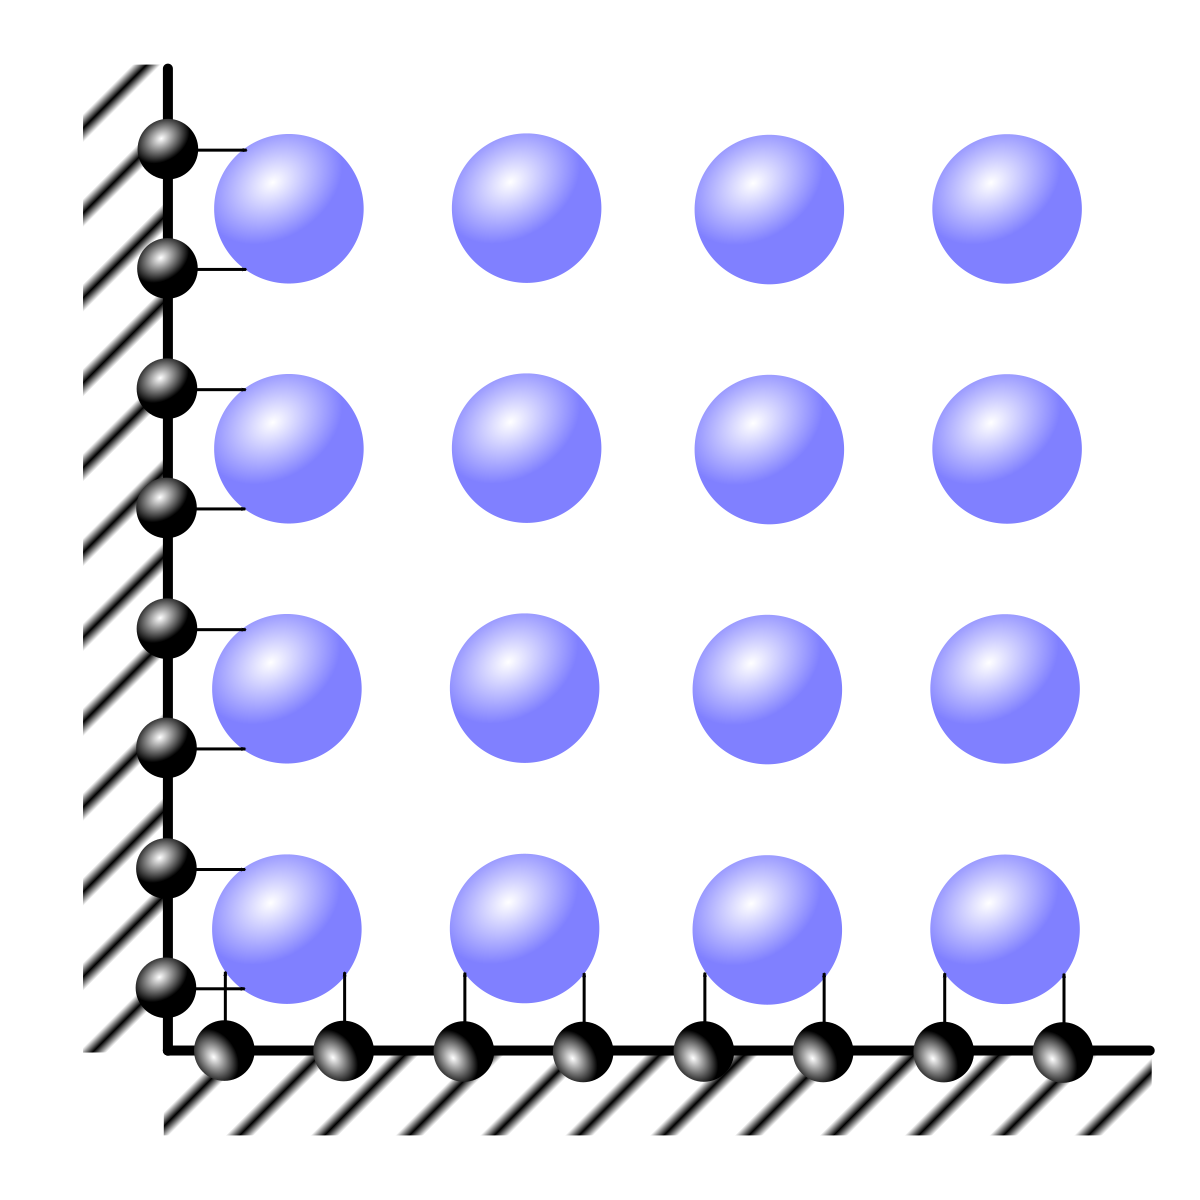
\includegraphics[width=0.4\textwidth]{DeLeffeCorner}
  \caption{Corner particles and vertexes distribution}
  \label{fig:aquagpusph:DeLeffeCorner}
\end{figure}
%